

\section{Unleash the Potential of RLVR and OPD}
\label{sec:motivation}


This section motivates CoPD through three steps. We first formalize the structural costs incurred by mixed-data RLVR and the static OPD pipeline under a unified framework, showing that each paradigm sacrifices part of the optimization signal in a different way (\S\ref{sec:moti-analysis}). We then hypothesize that effective OPD requires teacher and student to share similar behavioral patterns, and use top-$k$ token overlap as a measurable indicator of this property (\S\ref{sec:moti-hypothesis}). Finally, we verify both the indicator and its implications through a pilot study, which directly motivates the design of CoPD (\S\ref{sec:moti-pilot}).

\subsection{A Unified View of Existing Paradigms}
\label{sec:moti-analysis}

We consider the problem of consolidating two capabilities, represented by datasets $D_1$ and $D_2$, into a single unified policy. Let $X(D_1, D_2)$ denote the total optimization signal contained in the two datasets, that is, the capability gain that would be realized if the signal from each dataset could be perfectly applied to the unified policy. We analyze each paradigm by how much of $X$ it actually delivers, and what additional cost it incurs. The resulting utility takes the schematic form
\begin{equation}
U_{\mathcal{P}} \;\approx\; a_{\mathcal{P}} \cdot X(D_1, D_2) \;+\; b_{\mathcal{P}},
\label{eq:utility-general}
\end{equation}
where $a_{\mathcal{P}} \in [0, 1]$ measures how effectively paradigm $\mathcal{P}$ converts $X$ into actual capability, and $b_{\mathcal{P}} \le 0$ captures any additional loss the paradigm incurs beyond imperfect conversion.

\paragraph{Mixed-data RLVR: capability divergence as conflict.}
When a single model is jointly optimized on $D_1 \cup D_2$, the per-step update averages the gradients induced by the two datasets. Because distinct capabilities favor different optimization directions, their gradients disagree on capability-specific dimensions, and the disagreement manifests as gradient conflict within each parameter update. The resulting utility takes the form
\begin{equation}
U_{\text{mix}} \;\approx\; X(D_1, D_2) \;-\; \Phi(D_1, D_2),
\label{eq:utility-mix}
\end{equation}
where $\Phi(D_1, D_2) > 0$ is the \textit{capability divergence cost}, the magnitude of the conflict between the two capabilities' optimization directions. Mixed-data RLVR pays this cost as the seesaw effect: gains on one capability are partially or fully canceled by interference from the other, no matter how the data mixing ratio is tuned. In Eq.~\eqref{eq:utility-general}, this corresponds to $a_{\text{mix}} = 1$ and $b_{\text{mix}} = -\Phi < 0$.

\paragraph{Static OPD pipeline: divergence avoided, but absorption is poor.}
The static pipeline avoids gradient conflict by training each expert in isolation, so each branch optimizes its own gradient without interference and the divergence cost $\Phi$ is removed. The cost is instead paid at the consolidation stage. An OPD step trains the student on its own on-policy trajectories $y \sim \pi_\theta(\cdot \mid x)$, with teacher $\pi_T$ providing token-level supervision at each visited state $y_{<t}$:
\begin{equation}
\mathcal{L}_{\text{OPD}}(\theta) = \mathbb{E}_{x, \, y \sim \pi_\theta} \left[ \frac{1}{|y|} \sum_{t=1}^{|y|} D_{\mathrm{KL}}\big(\pi_T(\cdot \mid x, y_{<t}) \,\|\, \pi_\theta(\cdot \mid x, y_{<t})\big) \right].
\label{eq:opd}
\end{equation}
We argue that the supervision in Eq.~\eqref{eq:opd} is most effective when teacher and student behave similarly along on-policy trajectories: their token-level distributions then overlap substantially, and the teacher's predictions reinforce tokens the student is already likely to produce. When experts have been trained to convergence in isolation, however, their behavior has drifted far from the shared base, and their predictions on the student's trajectories diverge sharply from the student's own. The OPD signal becomes hard to absorb under this mismatch, and only a small fraction of the optimization signal is transferred. The resulting utility takes the form:
\begin{equation}
U_{\text{static}} \;\approx\; \eta(\mathcal{O}_{\text{low}}) \cdot X(D_1, D_2),
\label{eq:utility-static}
\end{equation}
where $\eta(\mathcal{O}) \in [0, 1]$ is an absorption-efficiency function depending on teacher--student behavioral overlap $\mathcal{O}$, and $\mathcal{O}_{\text{low}}$ denotes the low overlap that arises after experts converge in isolation. In Eq.~\eqref{eq:utility-general}, this corresponds to $a_{\text{static}} = \eta(\mathcal{O}_{\text{low}})$, which is positive but small, and $b_{\text{static}} = 0$.

\paragraph{What CoPD aims to achieve.}
The two paradigms above sacrifice the optimization signal in opposite ways. Mixed-data RLVR delivers the full signal but pays a divergence cost; the static OPD pipeline removes the divergence cost but delivers only a small fraction of the signal. A paradigm that avoids both costs must satisfy two conditions simultaneously: (i) keep capability-specific optimization separated to remove the divergence cost, and (ii) maintain teacher--student overlap at a level where $\eta(\mathcal{O})$ is high so that the optimization signal can actually be absorbed. CoPD instantiates both conditions by alternating capability-specific RLVR with cross-branch mutual OPD, and its utility takes the form
\begin{equation}
U_{\text{CoPD}} \;\approx\; \eta(\mathcal{O}_{\text{mod}}) \cdot X(D_1, D_2), \quad \eta(\mathcal{O}_{\text{mod}}) \gg \eta(\mathcal{O}_{\text{low}}),
\label{eq:utility-copd}
\end{equation}
where $\mathcal{O}_{\text{mod}}$ is the moderate overlap actively maintained by the alternating structure. The static pipeline and CoPD share the same functional form: both remove the divergence cost ($b = 0$) and deliver $\eta(\mathcal{O}) \cdot X$, differing only in the value of $\mathcal{O}$ at which OPD operates. The remainder of this section grounds these claims empirically: \S\ref{sec:moti-hypothesis} introduces a measurable indicator of $\mathcal{O}$, and \S\ref{sec:moti-pilot} shows that $\eta$ does increase with $\mathcal{O}$ and that the static pipeline systematically operates at low $\mathcal{O}$.

\subsection{A Behavioral Hypothesis and a Measurable Indicator}
\label{sec:moti-hypothesis}

The analysis above identifies the absorption-efficiency function $\eta(\mathcal{O})$ as the key determinant of OPD effectiveness, and reduces the difference between the static pipeline and CoPD to the value of $\mathcal{O}$ at which each operates. To make this analysis testable, we need a measurable indicator of $\mathcal{O}$. We posit the following hypothesis.

\begin{tcolorbox}[colback=gray!8, colframe=gray!50, boxrule=0.5pt, arc=2pt]
\textbf{Behavioral consistency hypothesis.} An OPD signal is more easily absorbed when teacher and student exhibit more similar behavioral patterns, since their on-policy trajectories then visit similar states and the teacher's predictions agree more closely with the tokens the student is likely to produce.
\end{tcolorbox}

We instantiate this notion of behavioral similarity through the \textit{top-$k$ token overlap} along on-policy trajectories. Given a teacher $\pi_T$ and a student $\pi_\theta$, we define
\begin{equation}
\mathcal{O}_k(\pi_\theta, \pi_T) = \mathbb{E}_{x, \, y_{<t} \sim \mu_\theta} \left[ \frac{|\mathrm{Top}_k(\pi_\theta(\cdot \mid x, y_{<t})) \cap \mathrm{Top}_k(\pi_T(\cdot \mid x, y_{<t}))|}{k} \right],
\label{eq:overlap}
\end{equation}
where $\mathrm{Top}_k(\cdot)$ denotes the set of $k$ tokens with the highest predicted probability and $\mu_\theta$ is the state visitation distribution induced by the student. Larger $\mathcal{O}_k$ indicates that, at the states the student actually visits during generation, teacher and student agree on which tokens are likely. The hypothesis above predicts that $\eta$ in Eq.~\eqref{eq:utility-static} and Eq.~\eqref{eq:utility-copd} should rise with $\mathcal{O}_k$, at least until $\mathcal{O}_k$ becomes so high that teacher and student are behaviorally indistinguishable and the supervision carries no new information.

\begin{figure*}[t]
  \centerline{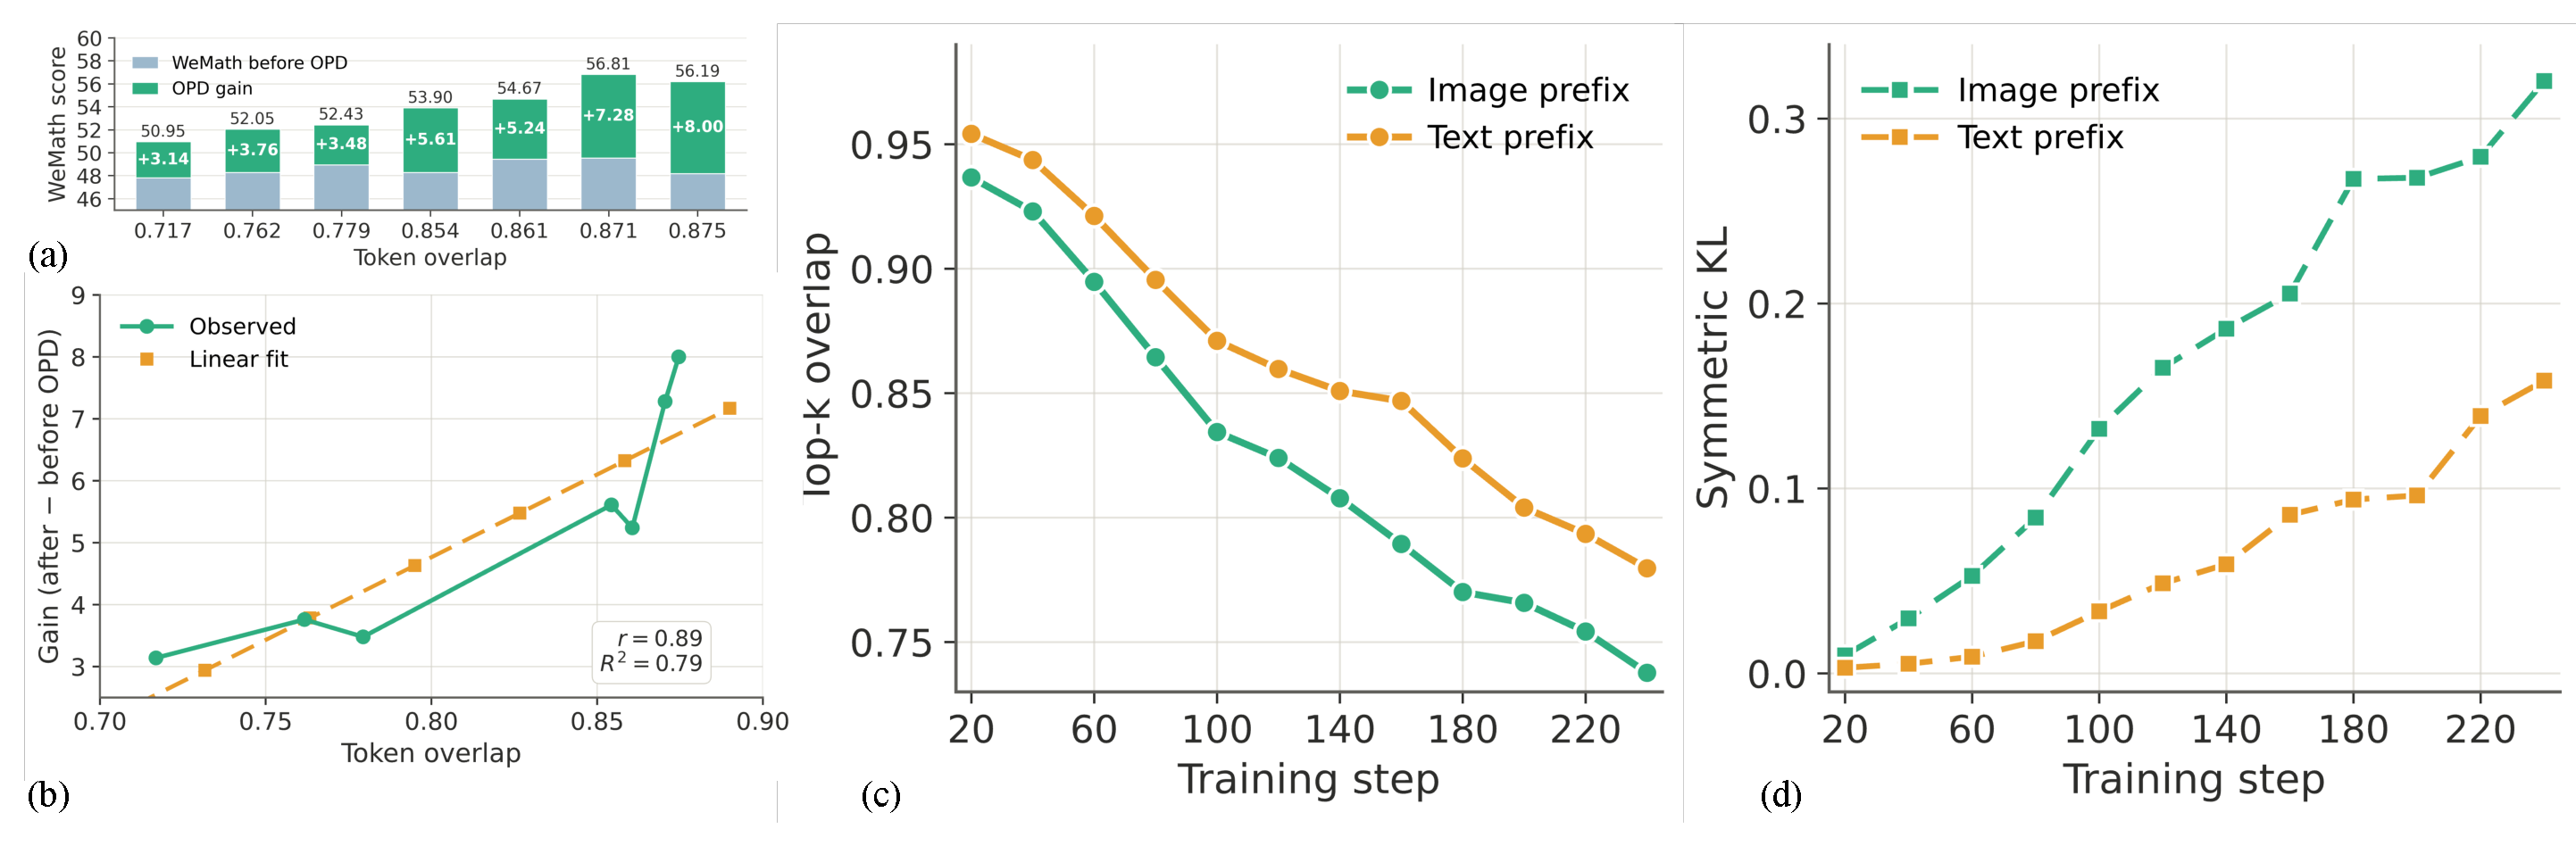
\includegraphics[scale=0.34]{figs/copd-pilot.pdf}}
  \vspace{-0.1cm}
  \caption{Pilot study motivating CoPD: post-OPD gain grows with teacher--student top-$k$ overlap, while standard RLVR training pushes overlap in the opposite direction. \textbf{(a)} WeMath score before and after OPD across student checkpoints with different top-$k$ overlap to the teacher; the OPD gain (green) increases with overlap. \textbf{(b)} The post-OPD gain plotted against top-$k$ overlap, with linear fit yielding $r=0.89$ and $R^2=0.79$. \textbf{(c)} As RLVR training proceeds, top-$k$ overlap drops and symmetric KL rises, consistently across image and text branches, indicating that experts trained to convergence drift outside the effective range identified in (a) and (b).}
  % \caption{ (a) Motivation and (b) Performance of \textbf{D}ynamic \textbf{E}arly \textbf{E}xit in \textbf{R}easoning.  }
  \label{fig:pilot}
\end{figure*} 


\subsection{Pilot Study}
\label{sec:moti-pilot}

We verify the hypothesis through two complementary experiments, summarized in Figure~\ref{fig:pilot}. The first establishes that $\eta(\mathcal{O}_k)$ does rise with $\mathcal{O}_k$ within the regime where teacher and student differ; the second establishes that the static pipeline systematically operates at a low value of $\mathcal{O}_k$.

\paragraph{Experiment 1: $\eta$ rises with teacher--student overlap.} 
We fix a teacher (an image-domain expert obtained by RLVR on $D_{\text{img}}$) and construct a series of students with varying $\mathcal{O}_k$ to the teacher by training the base checkpoint for a short period with different sampling temperatures. For each student, we run OPD on $D_{\text{img}}$ with identical training configurations and a fixed budget, and report the WeMath score before and after distillation, with $k = 10$ in $\mathcal{O}_k$.

As shown in Figure~\ref{fig:pilot}(a) and (b), the post-OPD gain increases monotonically with $\mathcal{O}_k$ across the sampled overlap range, exhibiting a strong linear correlation of $r = 0.89$ and $R^2 = 0.79$. This directly supports the behavioral consistency hypothesis: even with the teacher fixed, more behaviorally aligned students absorb the OPD signal more effectively, that is, $\eta$ in Eq.~\eqref{eq:utility-static} grows with $\mathcal{O}_k$. We do not observe the predicted decline at $\mathcal{O}_k \to 1$ in Figure~\ref{fig:pilot}(b), as temperature variation cannot drive the student all the way to teacher-identical behavior, but the boundary condition is straightforward: when teacher and student become indistinguishable, $D_{\mathrm{KL}}(\pi_T \| \pi_\theta) \to 0$ in Eq.~\eqref{eq:opd} and OPD gain necessarily collapses to zero. This boundary has its own design implication: simply running OPD continuously is not enough, since teacher and student would converge in behavior and the supervisory signal would lose informativeness. An effective paradigm must therefore actively maintain a non-trivial behavioral gap between teacher and student, in addition to keeping the gap from growing too wide.


\paragraph{Experiment 2: standard RLVR drives behavioral overlap into the low-$\eta$ regime.}
We then ask whether the static pipeline keeps OPD within the high-$\eta$ regime. We train two independent experts via RLVR, one on text-reasoning data $D_{\text{txt}}$ and one on image-reasoning data $D_{\text{img}}$, both initialized from a shared base $\pi_0$, and at fixed intervals measure each expert's top-$k$ overlap and symmetric KL with $\pi_0$ along on-policy rollouts. Treating $\pi_0$ as a proxy for the eventual student in two-stage distillation, these quantities track how teacher--student behavioral distance evolves during independent RLVR.



As shown in Figure~\ref{fig:pilot}(c)(d), $\mathcal{O}_k$ with the shared base drops monotonically as RLVR proceeds, while symmetric KL rises by an order of magnitude over the same span; the trend is consistent across both branches. This is the mirror image of the $\mathcal{O}_k \to 1$ regime discussed in Experiment 1: there, vanishing $D_{\mathrm{KL}}(\pi_T \| \pi_\theta)$ leaves the teacher with nothing new to convey; here, the growing $D_{\mathrm{KL}}$ means the teacher carries substantially more capability-specific knowledge than the student possesses, but their behavioral overlap is too low for that knowledge to be absorbed during distillation. By the time experts converge, they have moved far enough from the shared base that their overlap is well below the levels at which $\eta$ was shown to be highest in Experiment 1. This is the value of $\mathcal{O}_{\text{low}}$ in Eq.~\eqref{eq:utility-static}, and it confirms that the static pipeline systematically operates in the low-$\eta$ regime.


\paragraph{Implications for method design.}
The two experiments together expose a structural inconsistency in the static pipeline and point to a more nuanced requirement for $\mathcal{O}_k$. Experiment 1 shows that $\eta(\mathcal{O}_k)$ rises with overlap when teacher and student differ, but necessarily collapses when they become indistinguishable; Experiment 2 shows that training experts in isolation drives overlap toward the low end, where $\eta$ is also small. To raise $\eta$ from $\eta(\mathcal{O}_{\text{low}})$ to $\eta(\mathcal{O}_{\text{mod}})$ as Eq.~\eqref{eq:utility-copd} envisions, an effective paradigm must therefore satisfy three coupled requirements: (i) distillation must occur \emph{during} expert training rather than after it, so that $\mathcal{O}_k$ does not have time to drift toward the low-$\eta$ regime; (ii) the teacher must continue to evolve as the student does, so that their behavioral overlap is actively maintained rather than left to drift; and (iii) capability-specific training must continue to push the two sides apart, so that the supervision retains information the student does not already possess. The next section instantiates these three requirements as CoPD: cross-branch mutual OPD addresses (i) and (ii) by making each branch a continuously updated teacher for the other, while alternating with branch-specific RLVR addresses (iii) by periodically opening up the behavioral gap that subsequent OPD will then close.